\chapter{実験2 : 病理画像データセットを用いた実験}
\section{概要}
MNISTの実験から,提案したクエリ選考基準は,既存手法よりもCNNにとって識別率向上に寄与するサンプルを選択できていることが確認できた.
本章では,本研究で提案するシステムを用いて実際に病理画像データセットに対して行った実験について説明する.

\section{実験設定}
\subsection{データセットについて}
本実験では,Camelyon Grand Challenge\cite{Camelyon17}にて公開されたCamelyonデータセットを利用した.
Camelyonデータセットは1000枚のWSIからなり,乳癌のリンパ節転移を自動で検出する識別器を生成することを目的としたデータセットである\todo{図}.
各WSIは一枚あたり100,000×100,000ピクセルの大きさで,細胞組織を含む画像パッチは約10,000から400,000枚になる.
また,それら全ての画像パッチに対して癌か正常かの二値のラベルが付与されている.
ここでも,MNISTで行った実験と同様に各画像パッチのラベルは,クエリとして問い合わせない限り与えられない状況とする.

\section{予備実験}
\todo{都合の良い特徴量とか識別器を使ってるのずるいのかな}

\subsection{クラスタリング手法の比較}
第3章で述べたクラスタリングに使用する特徴量を比較するために,それぞれの特徴量を用いて病理画像データセットをK-meansによってクラスタリングを行った際の
各クラスター内のラベルの不純度を平均を計算した.不純度が小さいほどクラスター内でのばらつきが小さく良い特徴量だと言える.
データセットは100,000枚の病理画像からなり,癌と正常の割合は均等に調整した.
使用したデータセットの詳細は第5章で説明する.
表\ref{table:compare_feat}に示すように,CNNを用いたテクスチャ特徴量であるCompact Bilinear Poolingをクラスタリングに用いるのが妥当であると考えられる.

\begin{table}[h]
  \caption{\label{table:compare_feat}比較実験の結果}
  \center
  \begin{tabular}{c|c} \hline
     手法 & Inpurity \\ \hline
    LBP & 0.396 \\
    CNNの中間特徴量 & 0.335  \\ 
    Compact Bilinear Pooling & $\textbf{0.330}$ \\ \hline
  \end{tabular}
\end{table}

\subsection{線形識別器との比較}
線形識別器による能動学習の研究は多数ある.
ここで,特徴量を固定し線形識別器で学習した場合と特徴量も同時に学習した場合の精度を比較するために,
病理画像データセットに対して実験を行った.
識別機に用いるCNNはGoogLeNet \cite{szegedy2015going}を採用した.
一般画像認識で利用される数多くのCNNアーキテクチャの中でも比較的計量で,
医療画像解析でしばしば用いられるモデルであることから選択した.

図\ref{table:compare_classifier}に示すように,特徴量に深層学習によって得られたものを使用した場合でも,
特徴量を同時に学習したものは線形識別器の精度を遥かに上回る結果となった.
また,通常のCNNよりも,Compact Bilinear Poolingによって空間の情報を落として
テクスチャ特徴量として扱ったほうが良い識別精度を達成することを確認した.

\begin{table}[h]
  \caption{\label{table:compare_classifier}比較実験の結果}
  \center
  \begin{tabular}{c|c} \hline
    手法 & Accuracy  \\ \hline
    LBP + 線形SVM & 80.2 $\%$ \\
    CNNの中間特徴量 + 線形SVM & 84.4 $\%$  \\ 
    Compact Bilinear Pooling + 線形SVM & 86.0 $\%$ \\ \hline
    CNN + finetune & \textbf{94.1} $\%$  \\ 
    Compact Bilinear Pooling + finetune & \textbf{95.1} $\%$ \\ \hline
  \end{tabular}
\end{table}


\section{実験の詳細}
予備実験から,識別機に用いるCNNはGoogLeNetの中間特徴をCompact Bilinear Poolingによって圧縮し全結合層を接続する構造とした.
以下に構造を示す(図\ref{figure:googlenet_cbp}).
\begin{figure}[tbp]
   \begin{center}
    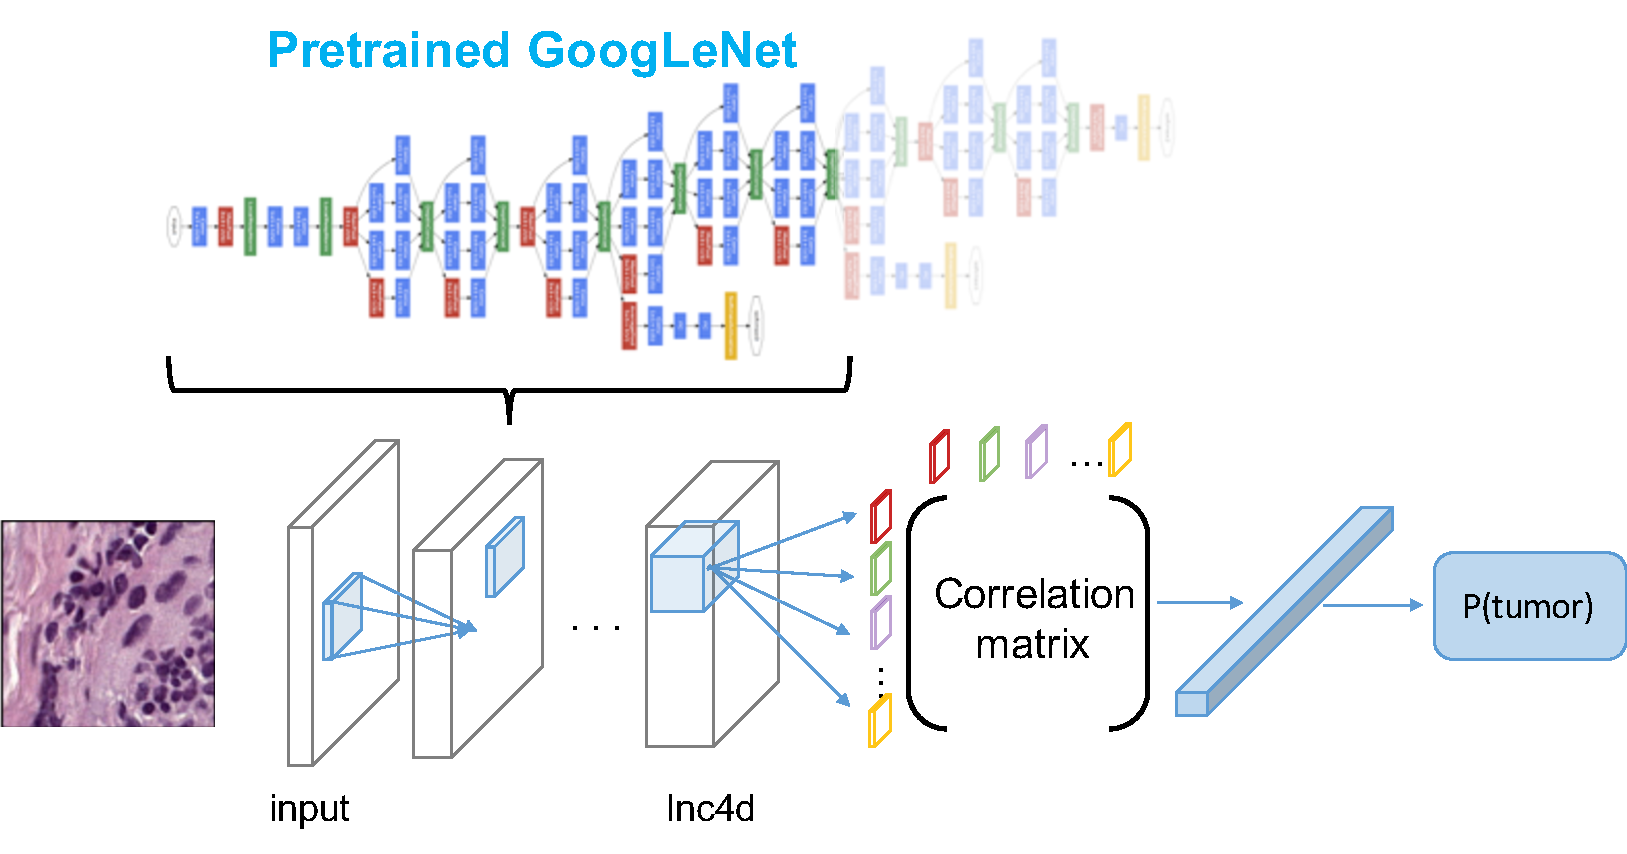
\includegraphics[width=12cm]{figures/googlenet_cbp.pdf}
   \end{center}
  \caption{\label{fig:googlenet_cbp}GoogLeNetの特徴量をCompact Bilinear Poolingによって圧縮し,全結合層を接続した構造}
\end{figure}
少ないラベルで高精度を達成するために,ImageNetのpretrained-modelを初期値として,fine-tuningによって学習を行う.

訓練時に使用するWSIから全ての画像パッチを抽出すると約5,000,000枚に登る.これをラベルなしデータセット$\mathcal{U}$とし,
各クエリ問い合わせでは$\mathcal{U}$からサンプリングされた$\mathcal{U}_i$から選択する.
$\mathcal{U}_i$のサイズは50,000に設定した.

本実験でも,同一クエリ内での情報の重複を避けるためクラスタリングを行う.
予備実験より,クラスタリングに使用する特徴量はCompact Bilinear Poolingを用いたテクスチャ特徴量を採用する.
committeeサイズは10, k-meansのクラスター数$K$は1000,一度に選択するクエリ$\mathcal{Q}$のサイズは100に設定した.
本実験では,実用的な状況に近づけるため,Mnistでの実験のように各iterationでの学習回数を固定にせず
与えられた比較的小さいバリデーションセットの性能が変化しなくなるまで学習を続ける,という設定にした.
バリデーションセットのサイズは100とした.
また,クラスターの代表サンプルから無作為にサンプリングされた100個のサンプルにラベルを付与して学習初期のラベルつきデータとして実験を開始した.
各クエリ問い合わせ毎に10000枚のテストデータに対する識別精度を計測し,ラベルを付与されたデータが10000に到達するまで実験を続けた.
比較手法は,以下の3つを使用した.
\begin{itemize}
  \item Random Sampling
  \item QBDP+Uncertain Sampling
  \item QBDP+Uncertain Sampling+Aug
\end{itemize}
実験ごとのばらつきを考慮し,同一の実験を3回行いその平均と標準偏差を計算した.

\section{実験結果}
本項では上記で述べた実験の結果を示す.
クエリ選考基準として提案手法,比較手法それぞれを使用した際の,ラベル付きサンプル数の増加に対するテスト精度の変化のグラフを図\ref{fig:camelyon_acc_graph}に示す.
pretrained-modelからのfine-tuningを行っているため,若干不安定ながら少ないラベルでも学習が進んでいることがわかる.
Randomなベースラインと比較して,提案した手法は識別に有効なサンプルを選択できていることがわかる.
さらに,Mnistの実験時よりも,推論時のData Augmentationの利用の効果が顕著に現れていることがわかる.
それぞれのクエリ選考基準を利用して構築された1000枚のラベル付きデータセットを学習した識別精度と,ラベルを全て使った場合の識別精度の比較した図を表\ref{table:camelyon_last_accuracy}に示す.
表より,提案手法を用いた場合,全てのラベルを利用して達成される識別精度にはやや劣るものの,比較して遜色ない性能を,10,000枚のラベルで達成することができた.
これは,実際ラベル付きデータがパッチレベルでは数100万枚存在することを考慮すると,100分の1のラベル数で学習に成功したという事もできる.
最後に,ラベル付きデータセットが1000枚の際に,各手法によってクエリとして選択されたサンプルを図\ref{figure:camelyon_query_examples}に示す.

\begin{figure}[tbp]
     \begin{center}
      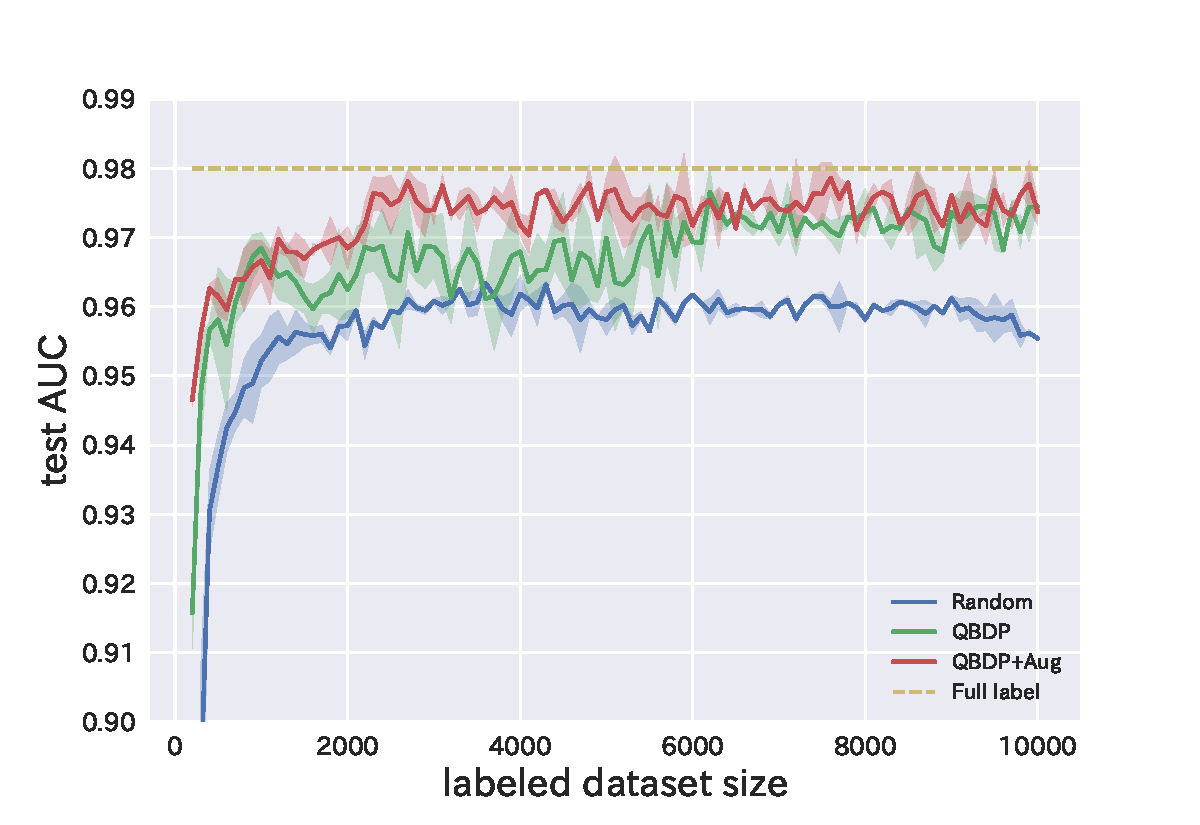
\includegraphics[width=12cm]{figures/camelyon_acc_graph.pdf}
     \end{center}
    \label{fig:camelyon_acc_graph}
    \caption{各手法を利用した場合のラベル付きサンプル数の増加に対するテスト精度の変化を示した図}
\end{figure}

\begin{table}[h]
  \caption{\label{table:camelyon_last_accuracy}それぞれのクエリ選考基準を利用して構築された1000枚のラベル付きデータセットを学習した識別精度と,ラベルを全て使った場合の識別精度の比較}
  \center
  \begin{tabular}{c|c} 
       &  AUC \\ \hline
      Random & 0.959 ± 0.002  \\
      Uncertain + QBC + Clustering & 0.972 ± 0.002  \\ 
      Uncertain + QBC + Clustering + DA & 0.975 ± 0.002  \\ \hline
      Full label (60000 label) & 0.98
  \end{tabular}
\end{table}

\begin{figure}[hbp]
  \begin{center}
      \subfloat[Random Sampling]{
        \scalebox{0.8}{
          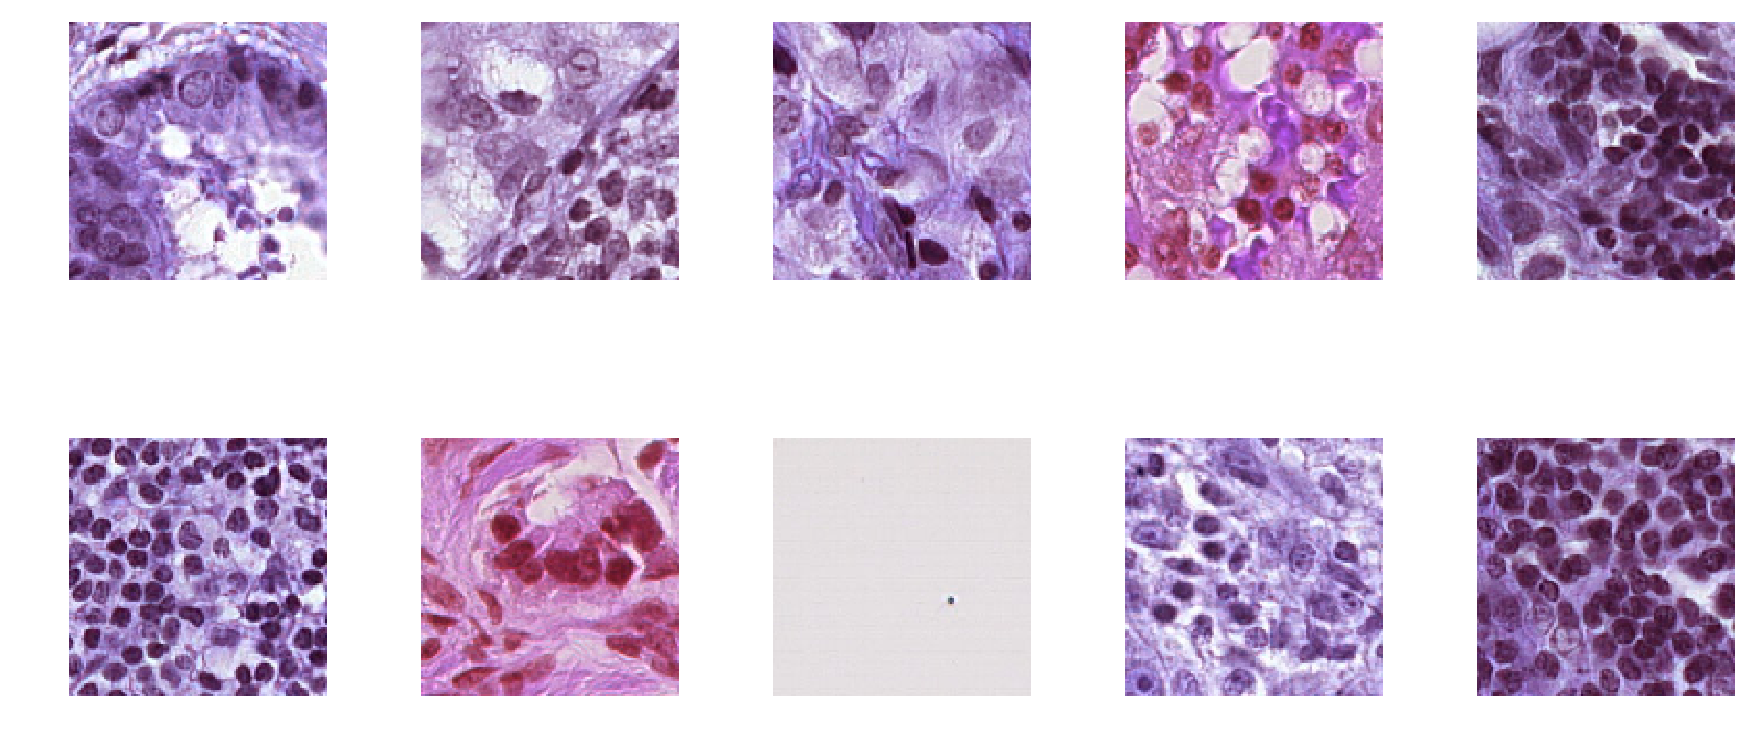
\includegraphics[width=8cm]{figures/camelyon_query_example_Random.pdf}
          }
      }

      \subfloat[Uncertain + QBDP]{
      \scalebox{0.8}{
          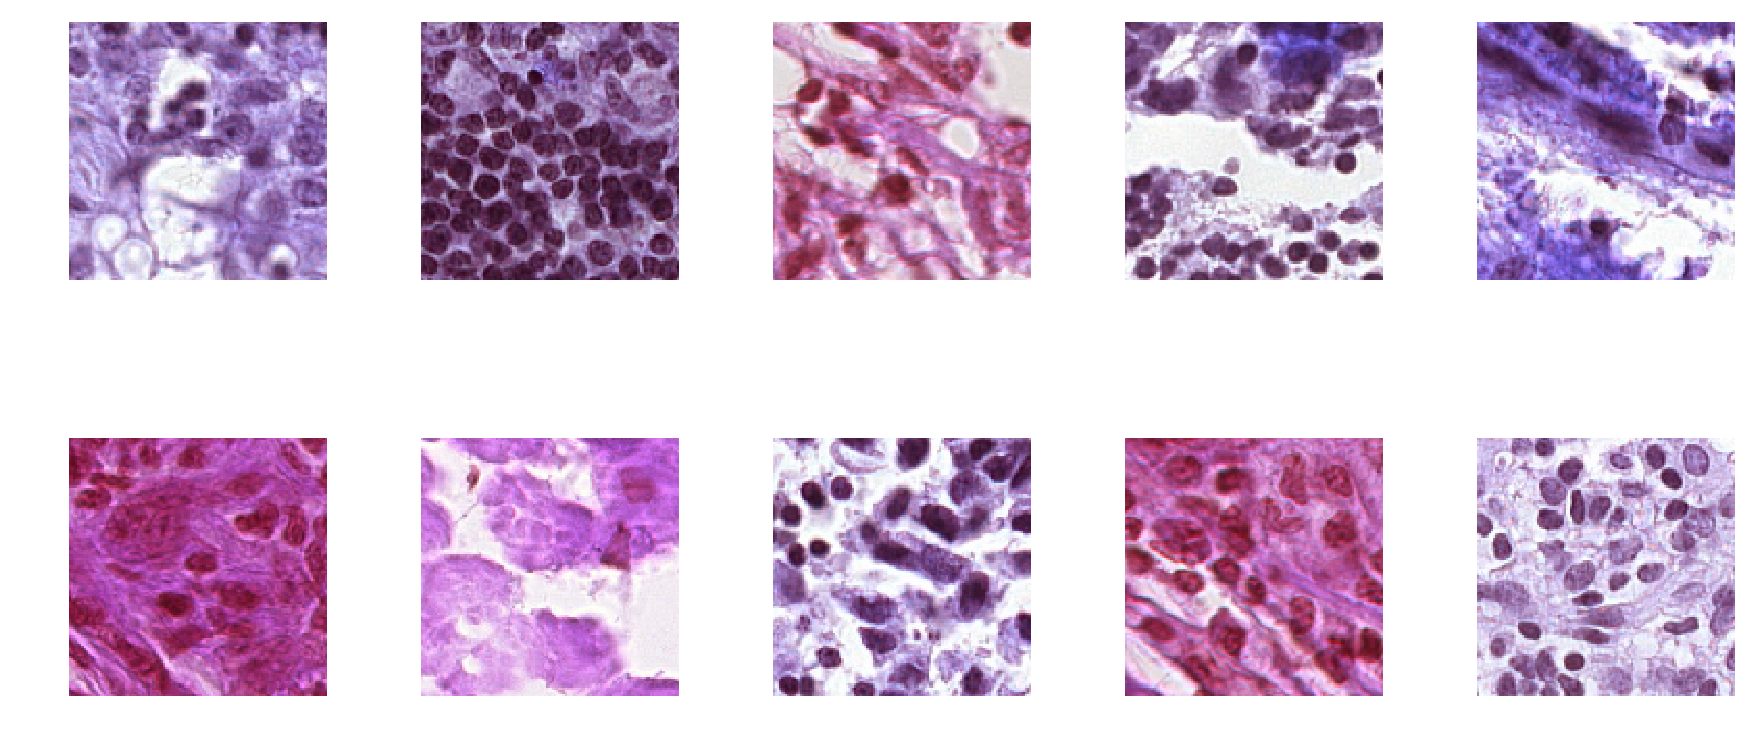
\includegraphics[width=8cm]{figures/camelyon_query_example_QBDP.pdf}
        }
      }
      \subfloat[Uncertain + QBDP + Aug]{
      \scalebox{0.8}{
      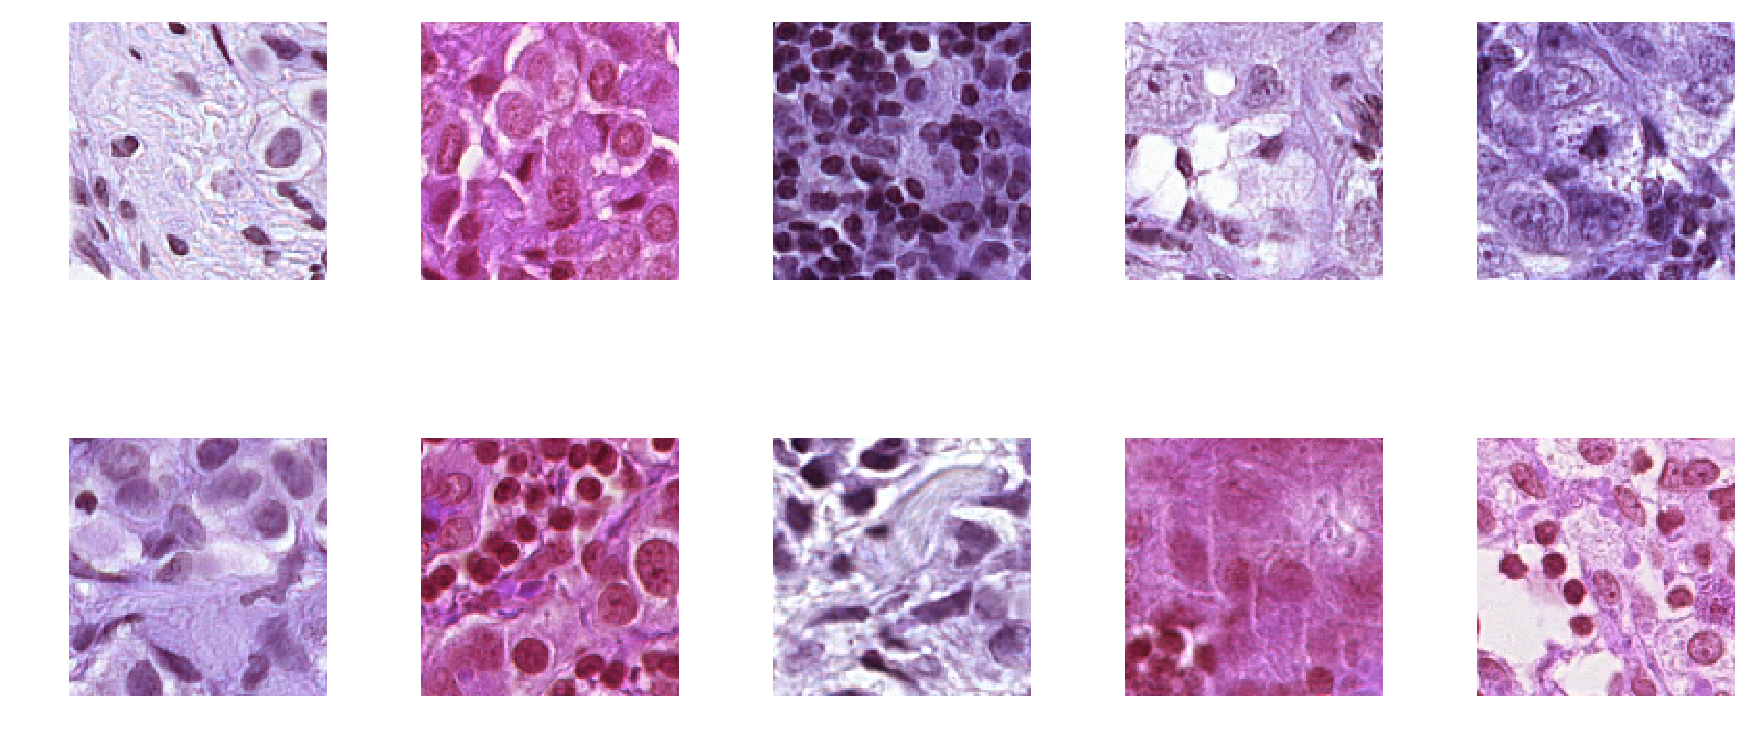
\includegraphics[width=8cm]{figures/camelyon_query_example_QBDP+Aug.pdf}
          }
      }
  \caption{\label{figure:camelyon_query_examples}各手法によってクエリとして選択されたサンプルを示す.}
  \end{center}
\end{figure}


\section{まとめ}
本研究で提案するシステムを大規模病理画像データセットに適用し,システムの有効性を検証した.
病理画像解析においてCNNを用いてテクスチャ特徴量を利用しながらfine-tuningすることで,他の手法よりも性能が良いことを実験で示した.
巨大なパラメータを持つCNNを採用し,識別精度を犠牲にすることなく,WSI全体の画像パッチ群と比較した場合アノテーションコストを1$\%$程度まで減らすことに成功した.
また,それらを現実的な計算コストで実現を可能とした.
